\documentclass{article}

\usepackage[T1]{fontenc}
\usepackage[spanish,es-tabla,es-noquoting,es-nodecimaldot]{babel}
\usepackage{csquotes}
\usepackage[letterpaper,top=2cm,bottom=2cm,left=3cm,right=3cm,marginparwidth=1.75cm]{geometry}
\usepackage{amsmath}
\usepackage{graphicx}
\usepackage{booktabs}
\usepackage{tabularx}
\usepackage{float}
\usepackage[section]{placeins}
\usepackage[colorlinks=true, allcolors=blue]{hyperref}
\usepackage[backend=biber, style=authoryear]{biblatex}
\addbibresource{references.bib}

\title{Clasificación supervisada de coberturas tras el colapso de la presa de Brumadinho (Minas Gerais, Brasil) con Sentinel-2\\[0.5em]
\large Proyecto final -- Fase 3: optimización, predicción y análisis}
\author{Jose Villarroel, Jose D. Medina, Camila Beltrán y Juan Rodríguez\\Pontificia Universidad Javeriana}
\date{\today}

\begin{document}

\maketitle

\begin{abstract}
Esta fase cierra el análisis comparativo de arquitecturas de aprendizaje automático para clasificar coberturas en Brumadinho. Se optimizaron los hiperparámetros de los seis modelos de la Fase~2 con validación cruzada agrupada por polígono, usando exclusivamente los 64 polígonos de entrenamiento; el test de 24 polígonos se mantuvo congelado. La búsqueda evaluó 224 combinaciones. La familia con mejor Kappa fue la regresión logística, pero el mejor candidato no fue estable; se eligió una configuración regularizada con pesos balanceados dentro de una desviación estándar del óptimo. En el test, el modelo final obtuvo una exactitud global de 94{,}7\,\% y un Kappa de 0{,}935, sin mejora demostrable frente a la Fase~2. El modelo se aplicó al ráster completo para generar un GeoTIFF temático con 74{,}10\,km$^2$ válidos: 42{,}19\,km$^2$ de vegetación densa, 17{,}76\,km$^2$ de vegetación baja, 4{,}65\,km$^2$ de relave, 7{,}94\,km$^2$ de urbano, 1{,}31\,km$^2$ de suelo expuesto y 0{,}26\,km$^2$ de agua. La clase relave incluye 2{,}85\,km$^2$ dentro del corredor y 1{,}80\,km$^2$ fuera de él, una limitación asociada a la confusión con superficies mineras desnudas. El mapa es una estimación basada en pseudo-etiquetas, no un inventario oficial.
\end{abstract}

\section{Contexto y objetivos}

La Fase~1 definió el evento, el área de estudio y la escena Sentinel-2 del 1 de febrero de 2019. La Fase~2 documentó el archivo \texttt{training\_dataset.tsv}, entrenó cinco modelos del enunciado más Random Forest y reportó las métricas iniciales. La Fase~3 tiene tres objetivos:

\begin{enumerate}
 \item optimizar los hiperparámetros de cada arquitectura con validación agrupada por polígono;
 \item seleccionar un modelo con un criterio fijado antes de mirar el test y evaluarlo una sola vez;
 \item aplicar el modelo a toda la imagen, generar el GeoTIFF temático, simbolizarlo en QGIS y cuantificar el área de cada clase.
\end{enumerate}

Este documento es el reporte separado de la Fase~3. Las Fases~1 y~2 se documentan en \texttt{report} y \texttt{report\_fase2}; el documento unificado de las dos primeras fases se conserva en \texttt{report\_completo}.

\section{Datos y protocolo}

El conjunto de entrenamiento contiene 1640 píxeles de 10\,m distribuidos en 88 polígonos y seis clases: vegetación densa, vegetación baja, agua, relave minero, suelo expuesto y urbano. La división de la Fase~2 se mantuvo sin cambios: 64 polígonos y 1168 píxeles para entrenamiento, 24 polígonos y 472 píxeles para prueba. Ningún polígono aparece en ambos conjuntos.

La Fase~3 no amplió ni reetiquetó el dataset. En particular, el polígono de suelo \texttt{5\_06}, que el modelo de la Fase~2 clasifica completo como urbano, se conserva en el test para no favorecer al modelo. La comparación con la versión de 72 polígonos se documenta por separado en \texttt{report\_fase2}; la prueba actual no es pareada con la anterior.

Se usó la pista oficial por píxel con las doce bandas espectrales. La pista B, basada en medianas por polígono, se conserva como análisis exploratorio de la Fase~2 y no se usa para el mapa final.

\section{Optimización de hiperparámetros}

\subsection{Protocolo}

La búsqueda se hizo solo con los 64 polígonos de entrenamiento, mediante \texttt{StratifiedGroupKFold} de cuatro pliegues con semilla 42 \parencite{Roberts2017}. La métrica de selección fue el Kappa medio; se registraron también F1 macro y exactitud balanceada. El test congelado no participó en la búsqueda ni en la selección.

Se evaluaron 224 combinaciones: 10 de regresión logística, 80 de árbol de decisión, 30 de Random Forest, 50 de SVM, 30 de red neuronal y 24 de KNN. Los espacios fueron:

\begin{itemize}
 \item LR: $C \in \{0{,}01, 0{,}1, 1, 10, 100\}$ y pesos \texttt{None}/\texttt{balanced};
 \item DT: profundidad, hojas mínimas, criterio y pesos;
 \item RF: 300/500 árboles, profundidad, hojas mínimas, variables por división y pesos balanceados;
 \item SVM: $C$, $\gamma$ y pesos;
 \item ANN: arquitectura, $\alpha$ y tasa de aprendizaje;
 \item KNN: $k$, pesos y distancia.
\end{itemize}

Los modelos se estandarizaron dentro de un \texttt{Pipeline} ajustado solo con cada pliegue de entrenamiento. Para evitar que un candidato con alta varianza entre pliegues se impusiera por una diferencia pequeña, se aplicó una regla de una desviación estándar: dentro de la familia ganadora se consideraron los candidatos con Kappa a menos de un error estándar del mejor; entre ellos se prefirieron los pesos balanceados y la menor desviación entre pliegues.

\subsection{Resultados de la búsqueda}

\begin{table}[htbp]
 \centering
 \small
 \setlength{\tabcolsep}{4pt}
 \caption{Mejor Kappa de validación agrupada por familia. La columna final marca la familia seleccionada.}
 \label{tab:hpo}
 \begin{tabular}{lcccc}
  \toprule
  Modelo & Kappa CV & F1 CV & Candidatos & Seleccionado \\
  \midrule
  LR & 0{,}938 & 0{,}956 & 10 & Sí \\
  SVM & 0{,}918 & 0{,}938 & 50 & No \\
  ANN & 0{,}915 & 0{,}938 & 30 & No \\
  KNN & 0{,}904 & 0{,}931 & 24 & No \\
  RF & 0{,}856 & 0{,}895 & 30 & No \\
  DT & 0{,}791 & 0{,}829 & 80 & No \\
  \bottomrule
 \end{tabular}
\end{table}


La regresión logística tuvo el mejor Kappa medio (0{,}938), seguida por SVM (0{,}918), ANN (0{,}915), KNN (0{,}904), RF (0{,}856) y DT (0{,}791). La diferencia entre LR y SVM es de dos puntos porcentuales, pero la desviación entre pliegues también es apreciable y el test tiene solo 24 polígonos.

El mejor candidato de LR fue $C=100$ sin pesos balanceados, con Kappa 0{,}938 y una desviación de 0{,}066. Ese candidato tiene un Kappa de entrenamiento de 1{,}000 y una alta varianza; no se consideró una base estable. Dentro de una desviación estándar, la configuración $C=1$ con \texttt{class\_weight=balanced} quedó entre las más estables (Kappa 0{,}892, desviación 0{,}044) y fue la elegida. La Tabla~\ref{tab:params_finales} resume sus parámetros.

\begin{table}[htbp]
 \centering
 \small
 \setlength{\tabcolsep}{4pt}
 \caption{Hiperparámetros del modelo final (Regresión logística).}
 \label{tab:params_finales}
 \begin{tabular}{ll}
  \toprule
  Parámetro & Valor \\
  \midrule
  C & 1.0 \\
  class\_weight & balanced \\
  \bottomrule
 \end{tabular}
\end{table}


\begin{figure}[htbp]
 \centering
 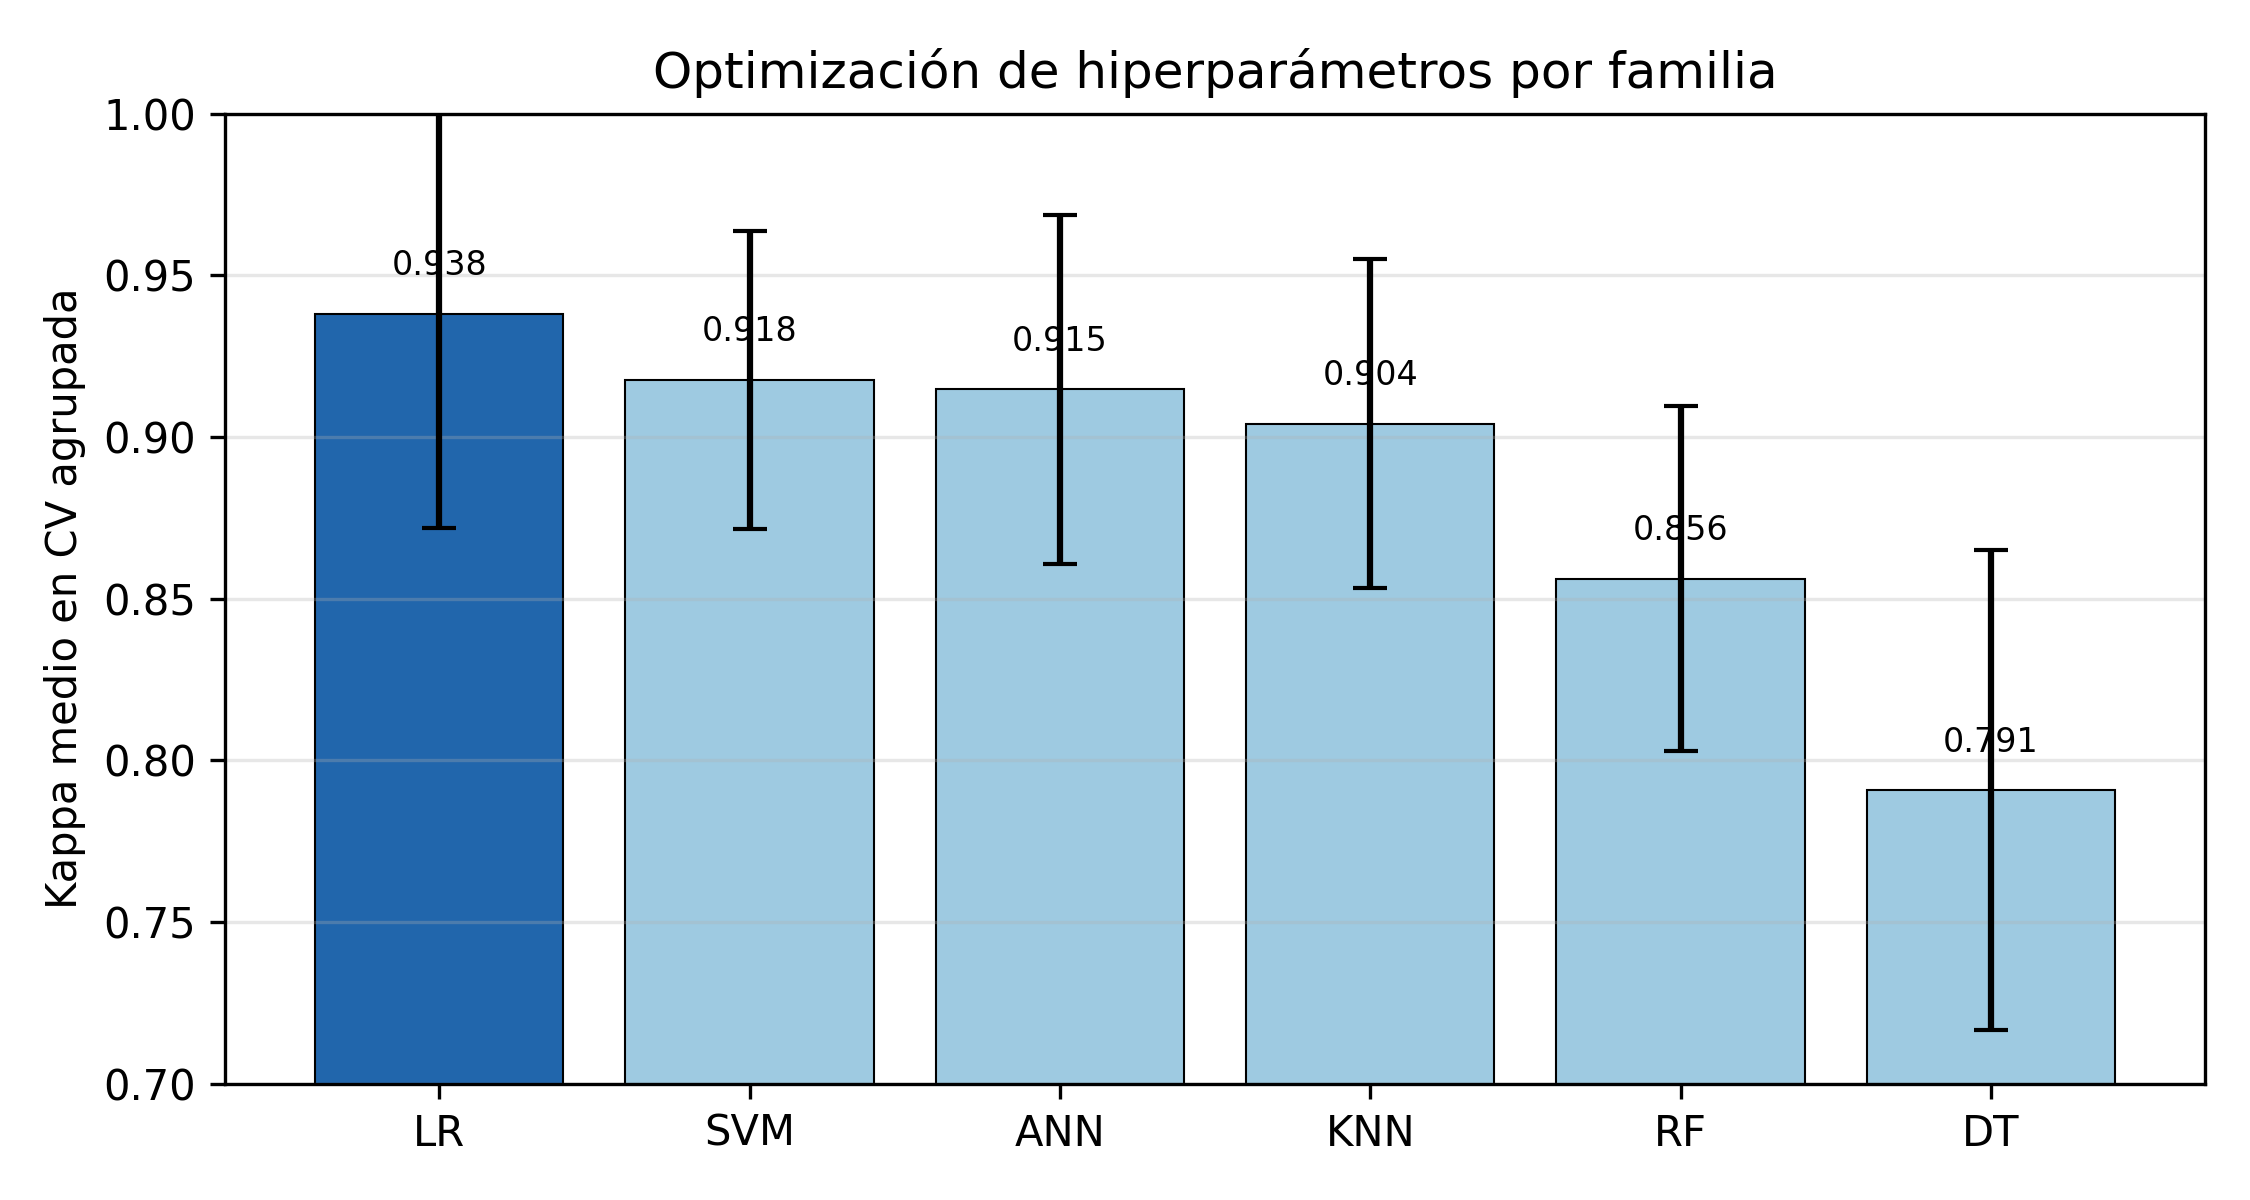
\includegraphics[width=0.82\textwidth]{figures/hpo_modelos.png}
 \caption{Kappa medio de la mejor configuración de cada familia en la validación agrupada. Las barras de error son la desviación estándar entre pliegues.}
 \label{fig:hpo}
\end{figure}

\section{Evaluación en el test congelado}

Los seis modelos tuneados se entrenaron con los 64 polígonos de entrenamiento y se evaluaron una sola vez en los 24 polígonos de prueba. La Tabla~\ref{tab:phase3_metricas} y la Figura~\ref{fig:tuned} resumen los resultados.

\begin{table}[htbp]
 \centering
 \small
 \setlength{\tabcolsep}{4pt}
 \caption{Métricas en el test congelado de 24 polígonos y Kappa de validación agrupada. \emph{CV familia} es el mejor Kappa de la familia; \emph{CV modelo} es el del conjunto de hiperparámetros elegido.}
 \label{tab:phase3_metricas}
 \begin{tabular}{lcccccc}
  \toprule
  Modelo & OA & Kappa & F1 & CV modelo & CV familia & Final \\
  \midrule
  LR & 0{,}947 & 0{,}935 & 0{,}933 & 0{,}892 & 0{,}938 & Sí \\
  RF & 0{,}917 & 0{,}899 & 0{,}910 & 0{,}856 & 0{,}856 & No \\
  ANN & 0{,}911 & 0{,}891 & 0{,}905 & 0{,}915 & 0{,}915 & No \\
  SVM & 0{,}890 & 0{,}865 & 0{,}888 & 0{,}918 & 0{,}918 & No \\
  KNN & 0{,}890 & 0{,}865 & 0{,}886 & 0{,}904 & 0{,}904 & No \\
  DT & 0{,}864 & 0{,}835 & 0{,}847 & 0{,}791 & 0{,}791 & No \\
  \bottomrule
 \end{tabular}
\end{table}


La regresión logística obtuvo la mejor exactitud global (0{,}947), el mejor Kappa (0{,}935) y el mejor F1 macro (0{,}933). Random Forest quedó en 0{,}917/0{,}899, la ANN en 0{,}911/0{,}891, SVM y KNN en 0{,}890/0{,}865, y el árbol de decisión en 0{,}864/0{,}835. La SVM, que en la Fase~2 empataba con LR, bajó al elegir un candidato con $C=100$; el resultado confirma que la búsqueda de hiperparámetros con 64 polígonos puede sobreajustar la validación.

\begin{figure}[htbp]
 \centering
 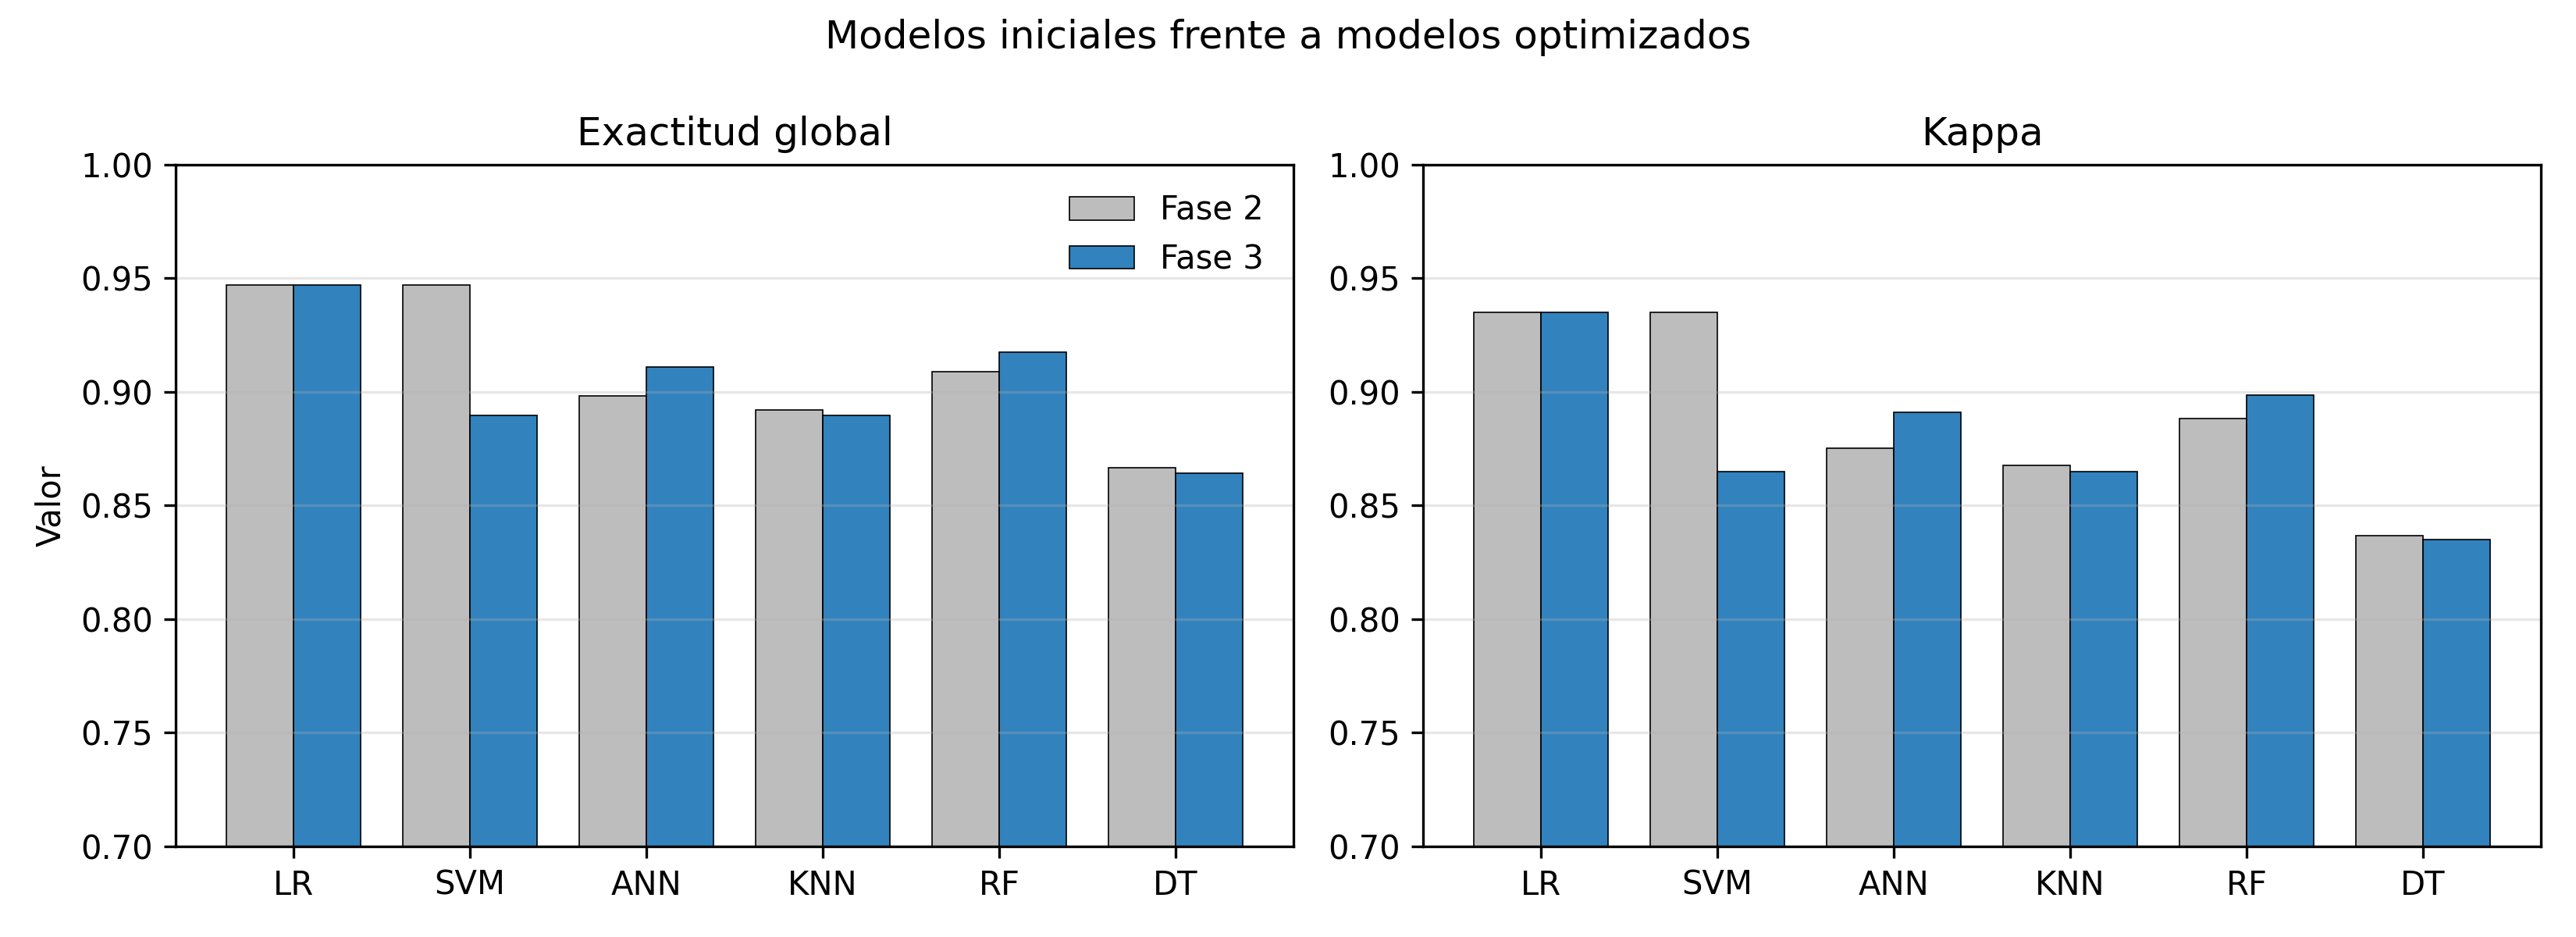
\includegraphics[width=\textwidth]{figures/tuned_vs_inicial.png}
 \caption{Exactitud global y Kappa de los modelos iniciales de la Fase~2 frente a los modelos optimizados de la Fase~3.}
 \label{fig:tuned}
\end{figure}

El modelo final no mejora el resultado de la Fase~2: la regresión logística mantiene 0{,}947 de exactitud y 0{,}935 de Kappa. La conclusión de la Fase~3 no es que el HPO haya mejorado el clasificador, sino que la configuración regularizada de LR es la opción más estable dentro de un conjunto pequeño y muy correlacionado.

\subsection{Matriz de confusión e importancia}

La Figura~\ref{fig:confusion} muestra la matriz de confusión del modelo final. Vegetación densa, vegetación baja, agua y relave se clasifican sin errores en el test. El único error es el polígono de suelo \texttt{5\_06}: sus 25 píxeles se asignan a urbano. Por eso el recall de suelo es 0{,}75 y la precisión de urbano es 0{,}59.

\begin{figure}[htbp]
 \centering
 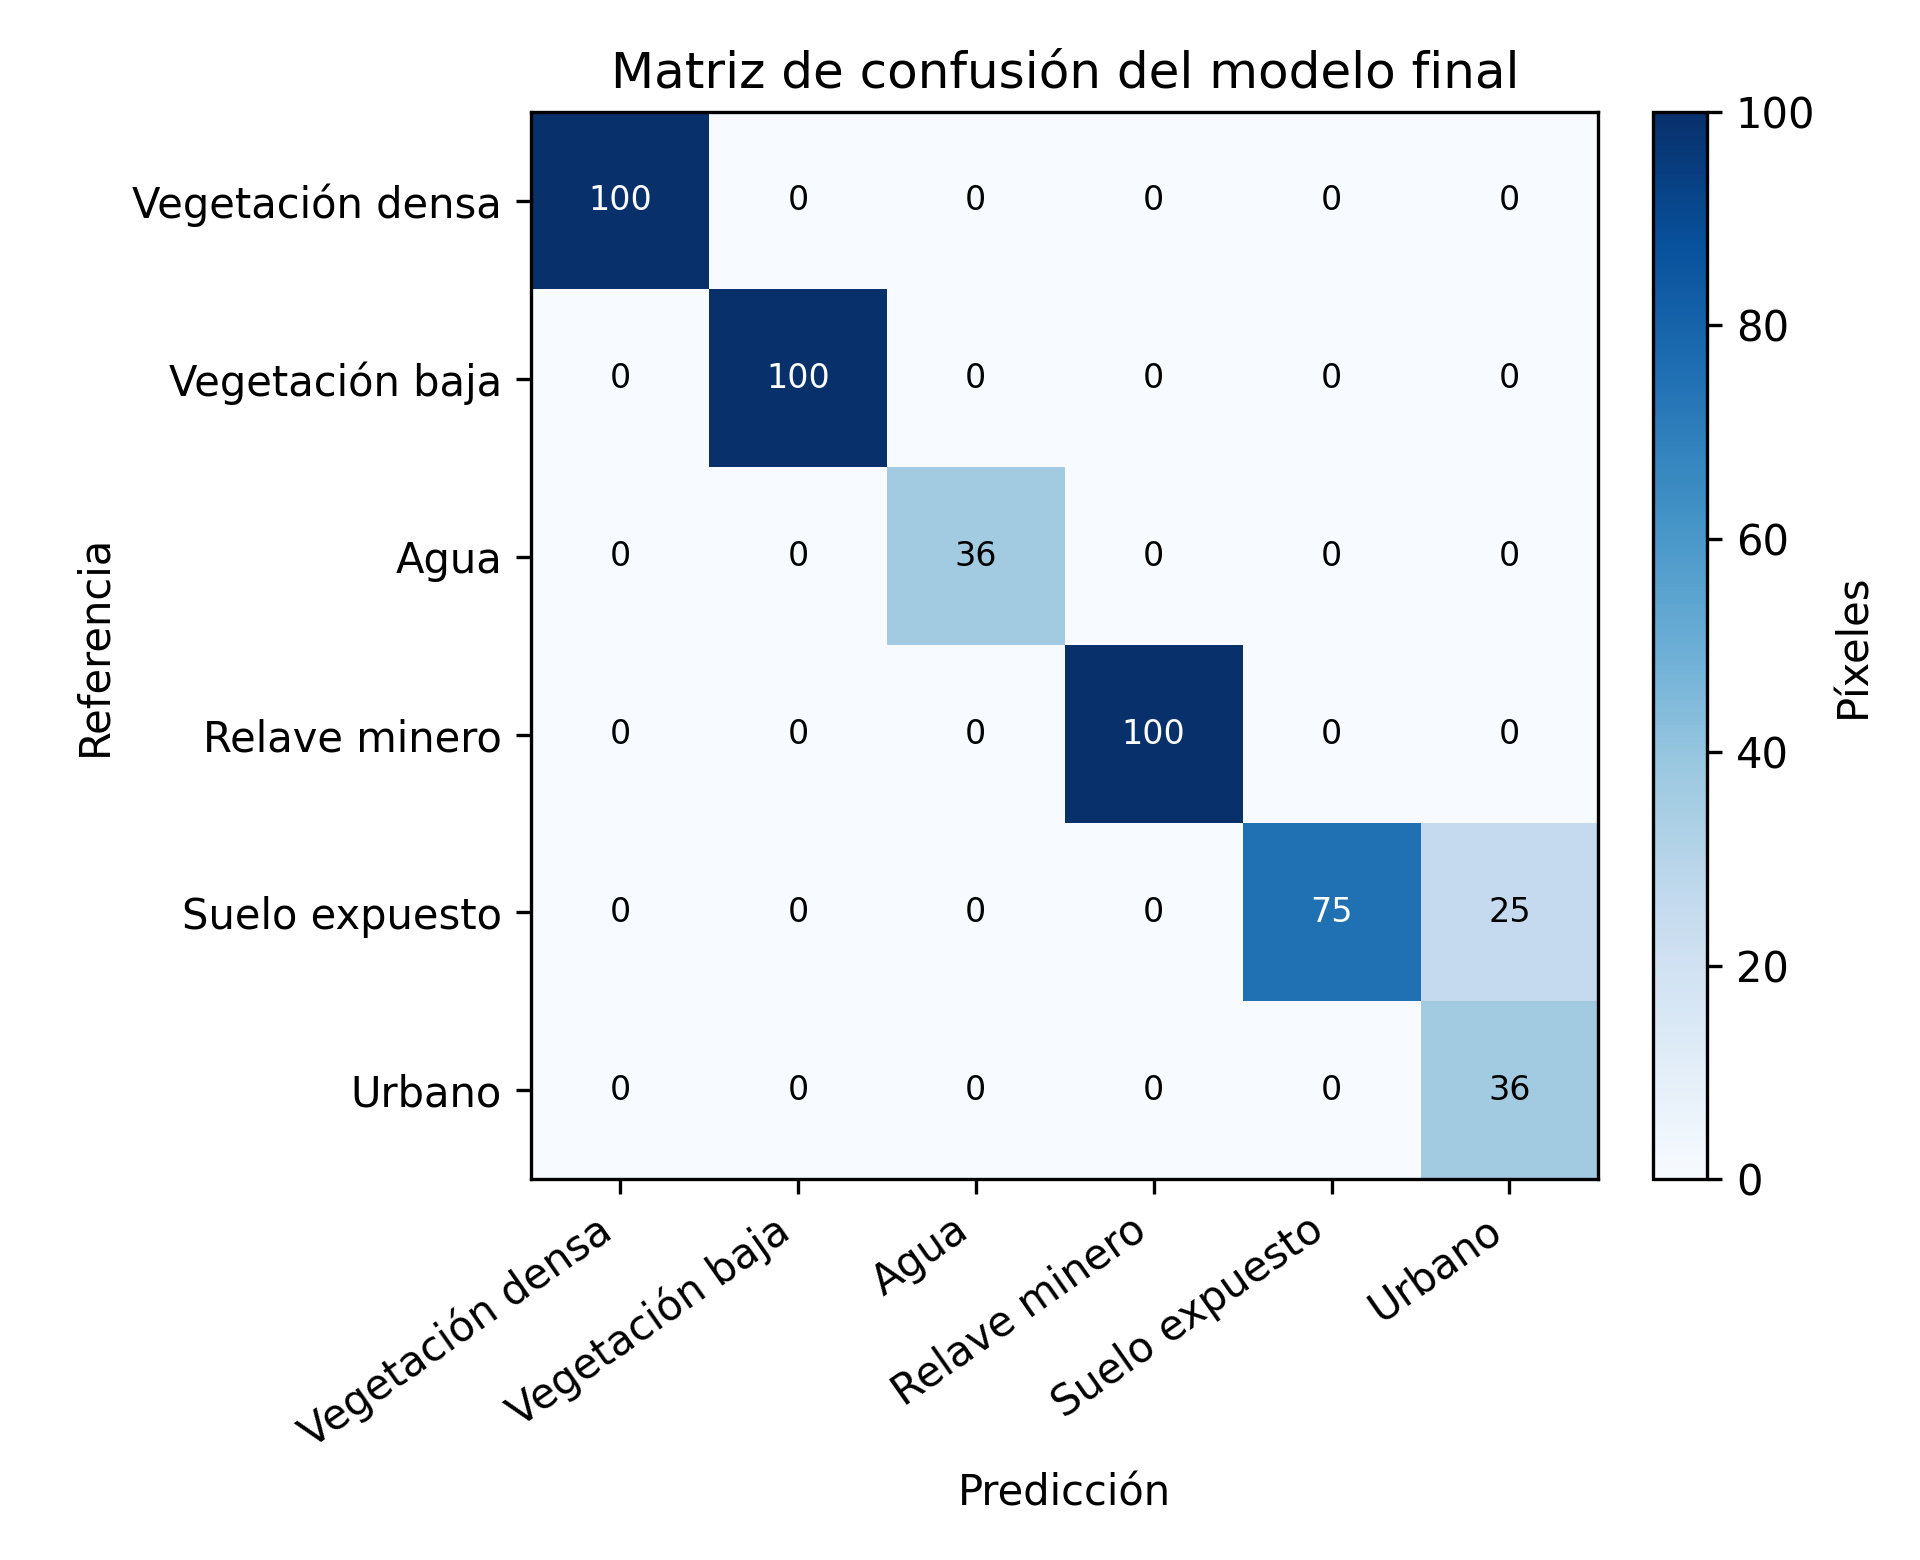
\includegraphics[width=0.72\textwidth]{figures/confusion_final.png}
 \caption{Matriz de confusión del modelo final sobre los 24 polígonos de prueba.}
 \label{fig:confusion}
\end{figure}

La Figura~\ref{fig:importance} presenta la importancia por permutación sobre el test. Las bandas B03, B09 y B02 concentran la mayor pérdida de exactitud al permutarse; B07, B8A y B08 aportan menos. Esta importancia es descriptiva: las bandas están correlacionadas y el test tiene 472 píxeles, por lo que no debe interpretarse como una prueba causal de la importancia espectral.

\begin{figure}[htbp]
 \centering
 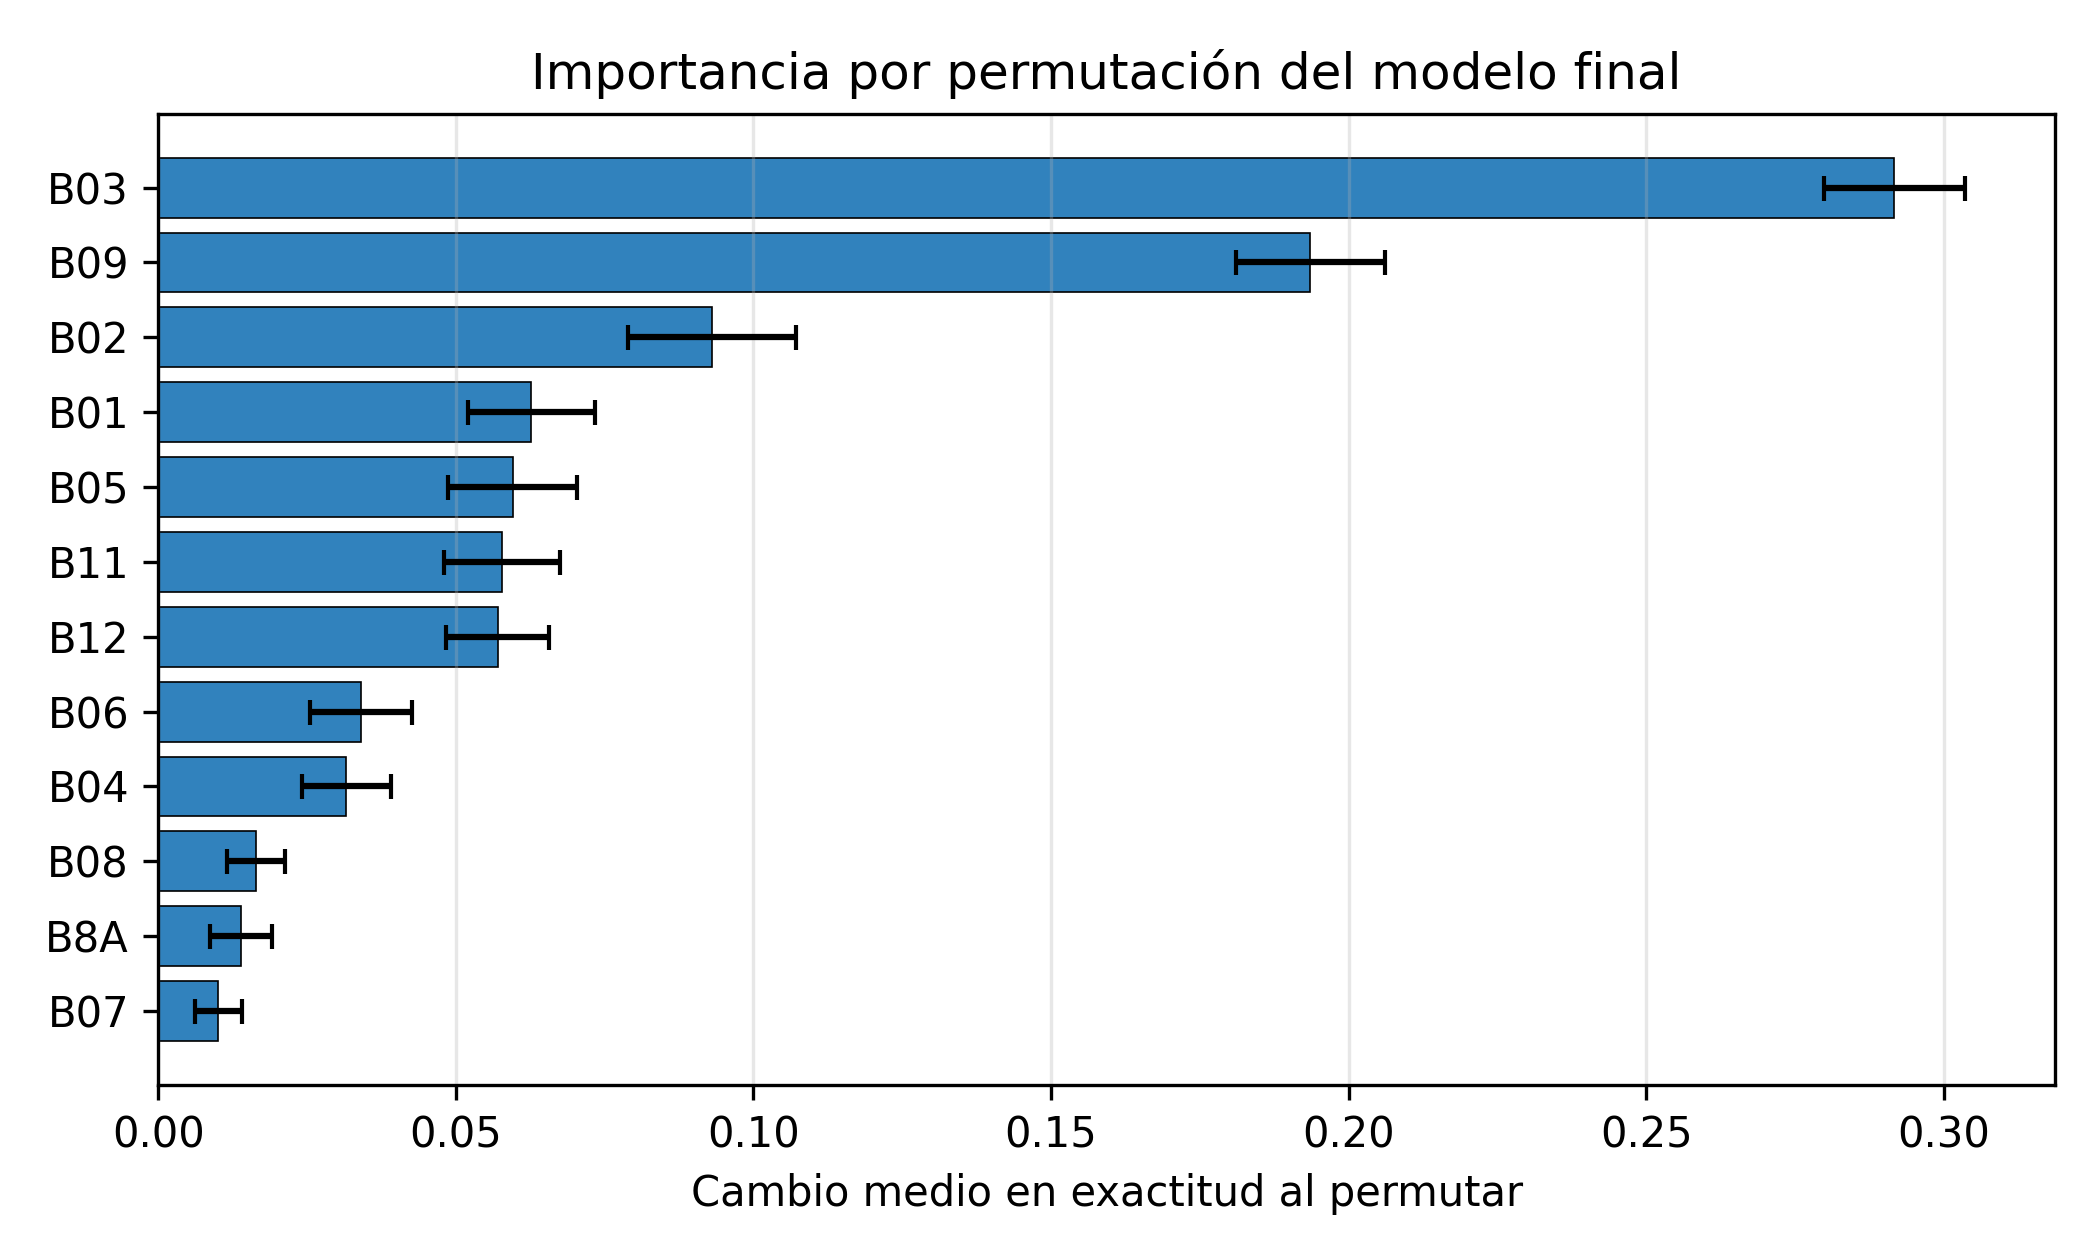
\includegraphics[width=0.8\textwidth]{figures/importancia_final.png}
 \caption{Importancia por permutación del modelo final. La barra es la media de 30 repeticiones y la línea el error estándar.}
 \label{fig:importance}
\end{figure}

\subsection{Incertidumbre y estabilidad}

El intervalo bootstrap del 95\,\% para la exactitud global del modelo final es 0{,}841--1{,}000; para Kappa, 0{,}809--1{,}000; para F1 macro, 0{,}815--1{,}000. La amplitud refleja que cada polígono de prueba pesa aproximadamente 5{,}3 puntos porcentuales. En la validación dejando un polígono fuera, la exactitud media fue 0{,}946 con error estándar 0{,}024, y el Kappa out-of-fold fue 0{,}912. Las diferencias entre modelos no deben interpretarse como superioridad definitiva.

\section{Inferencia y GeoTIFF temático}

El modelo final se reentrenó con los 88 polígonos y se aplicó al stack de doce bandas. La inferencia se hizo por bloques de 128 filas para no cargar todo el ráster. Antes de predecir se enmascararon:

\begin{itemize}
 \item los píxeles fuera de \texttt{study\_area.gpkg};
 \item los píxeles con SCL inválida: 0, 1, 3, 8, 9 y 10;
 \item los píxeles sin datos del stack.
\end{itemize}

El resultado es un GeoTIFF de una banda, tipo \texttt{uint8}, con el mismo CRS (EPSG:32723), el mismo \emph{transform}, ancho y alto que la imagen original. El valor 0 representa “sin datos”; 1--6 son las clases. El archivo incluye una tabla de colores y se acompaña de un estilo QGIS \texttt{.qml}.

\begin{figure}[htbp]
 \centering
 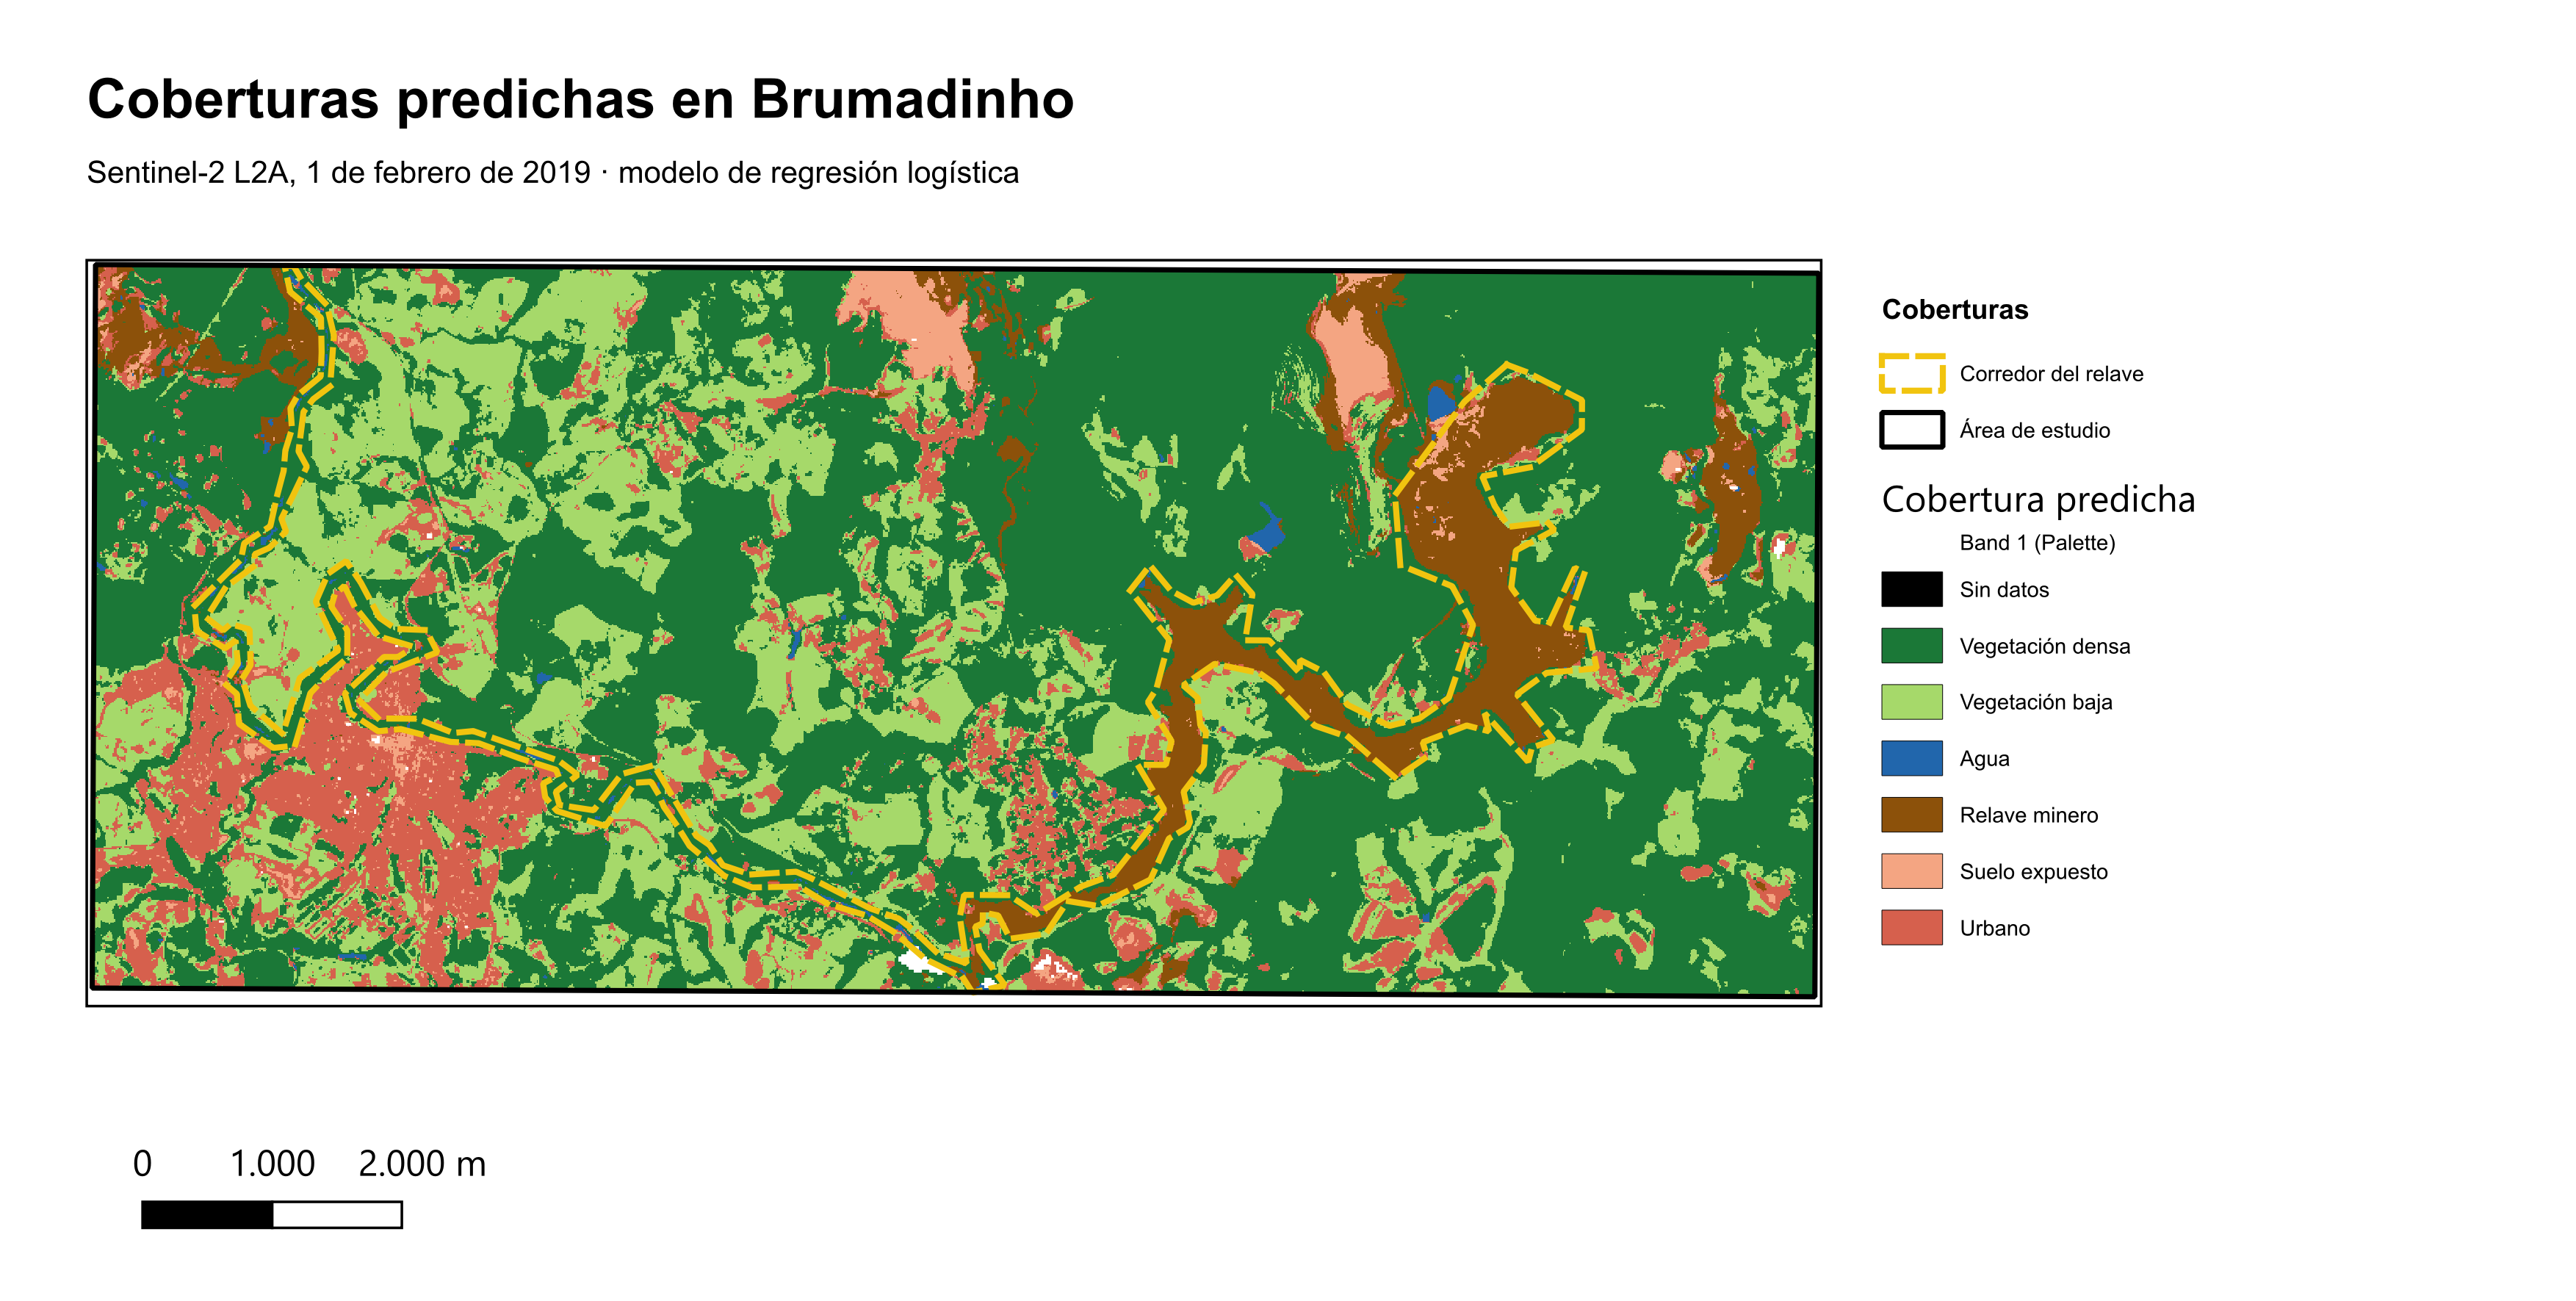
\includegraphics[width=\textwidth]{figures/mapa_tematico_qgis.png}
 \caption{Mapa temático exportado desde QGIS. El contorno negro delimita el área de estudio y la línea amarilla el corredor del relave.}
 \label{fig:mapa}
\end{figure}

El mapa se generó con QGIS 4.2.2 a partir del GeoTIFF y del estilo discreto. La Figura~\ref{fig:zoom} muestra el detalle del corredor del relave. La clase relave aparece a lo largo del corredor, pero también en zonas de la mina fuera de él; esa es una limitación de la separación espectral entre relave y suelo desnudo.

\begin{figure}[htbp]
 \centering
 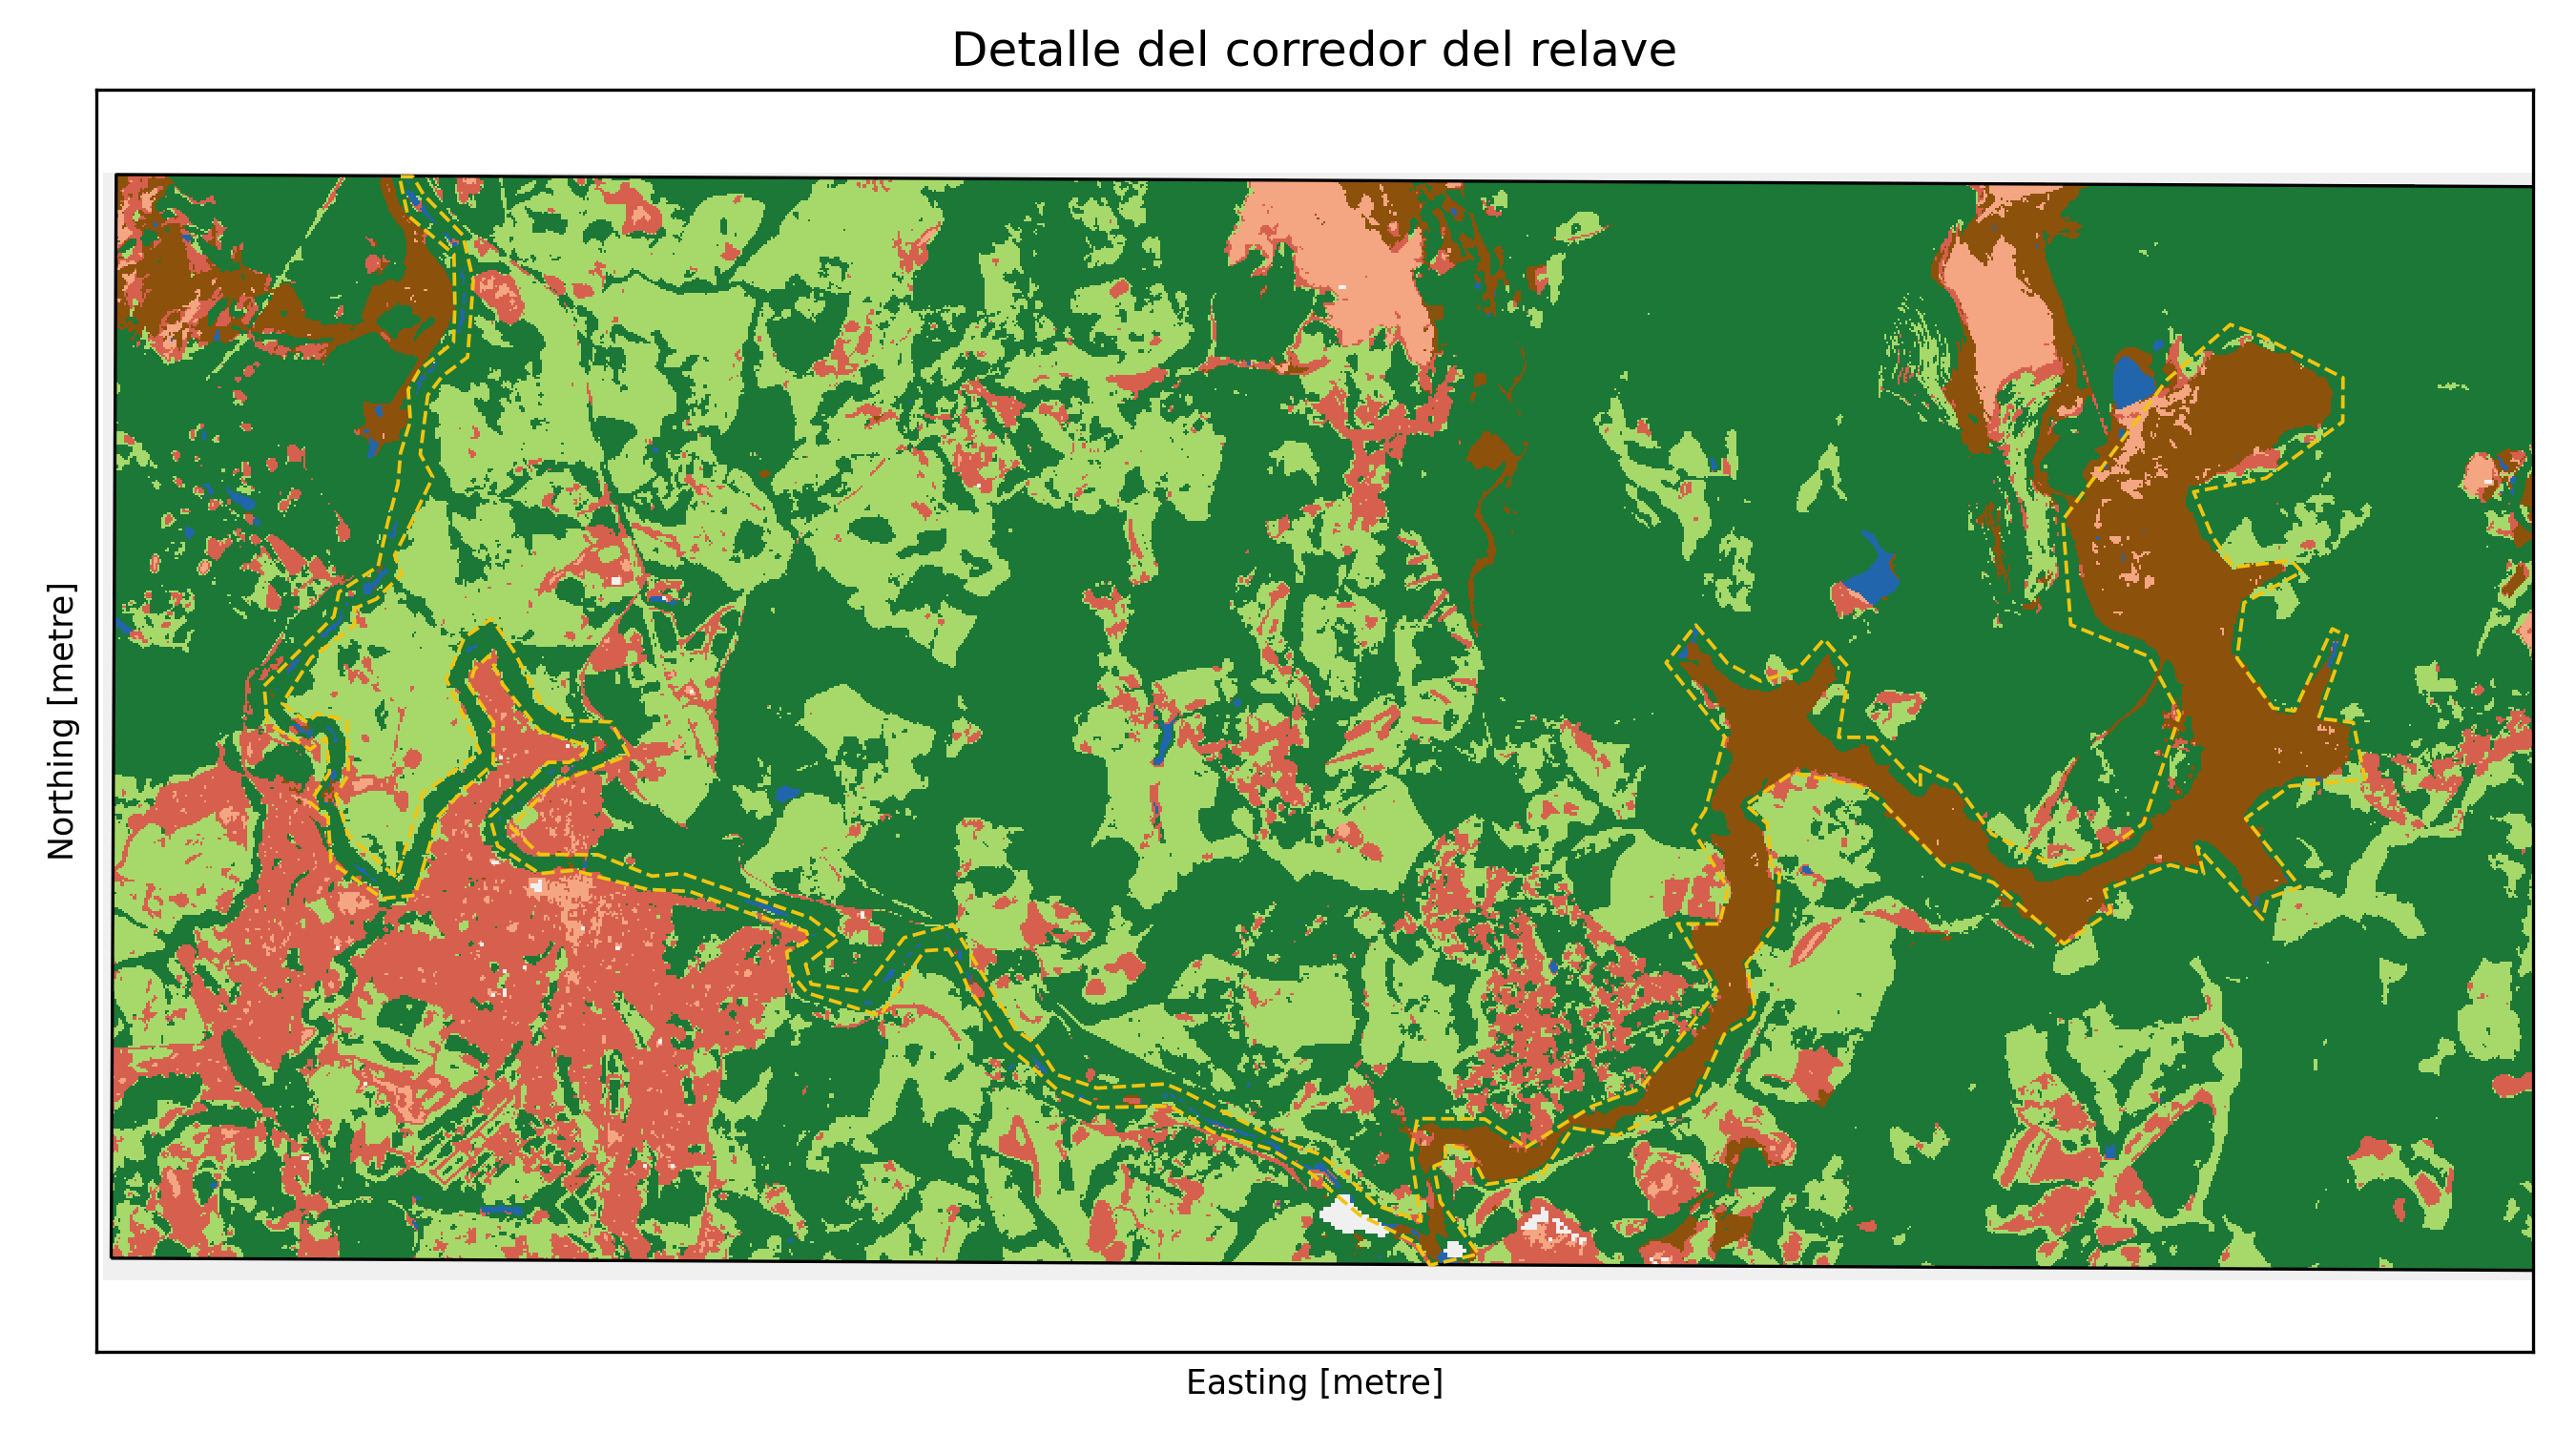
\includegraphics[width=0.9\textwidth]{figures/mapa_zoom_relave.png}
 \caption{Detalle del corredor del relave sobre el mapa predicho.}
 \label{fig:zoom}
\end{figure}

\section{Cuantificación de áreas}

La Tabla~\ref{tab:area_clases} resume las áreas predichas. El área válida total es 74{,}100\,km$^2$; los 2{,}166\,km$^2$ restantes son “sin datos” e incluyen el exterior del polígono de estudio y los píxeles inválidos por SCL.

\begin{table}[htbp]
 \centering
 \small
 \setlength{\tabcolsep}{4pt}
 \caption{Área predicha por clase. Los porcentajes se calculan sobre el área válida, no sobre el rectángulo completo.}
 \label{tab:area_clases}
 \begin{tabular}{lcccc}
  \toprule
  Clase & Píxeles & Hectáreas & km² & \% válido \\
  \midrule
  Vegetación densa & 421.852 & 4218{,}5 & 42{,}185 & 56{,}9\,\% \\
  Vegetación baja & 177.592 & 1775{,}9 & 17{,}759 & 24{,}0\,\% \\
  Agua & 2.605 & 26{,}1 & 0{,}261 & 0{,}4\,\% \\
  Relave minero & 46.498 & 465{,}0 & 4{,}650 & 6{,}3\,\% \\
  Suelo expuesto & 13.065 & 130{,}7 & 1{,}306 & 1{,}8\,\% \\
  Urbano & 79.388 & 793{,}9 & 7{,}939 & 10{,}7\,\% \\
  \bottomrule
 \end{tabular}
\end{table}


\begin{figure}[htbp]
 \centering
 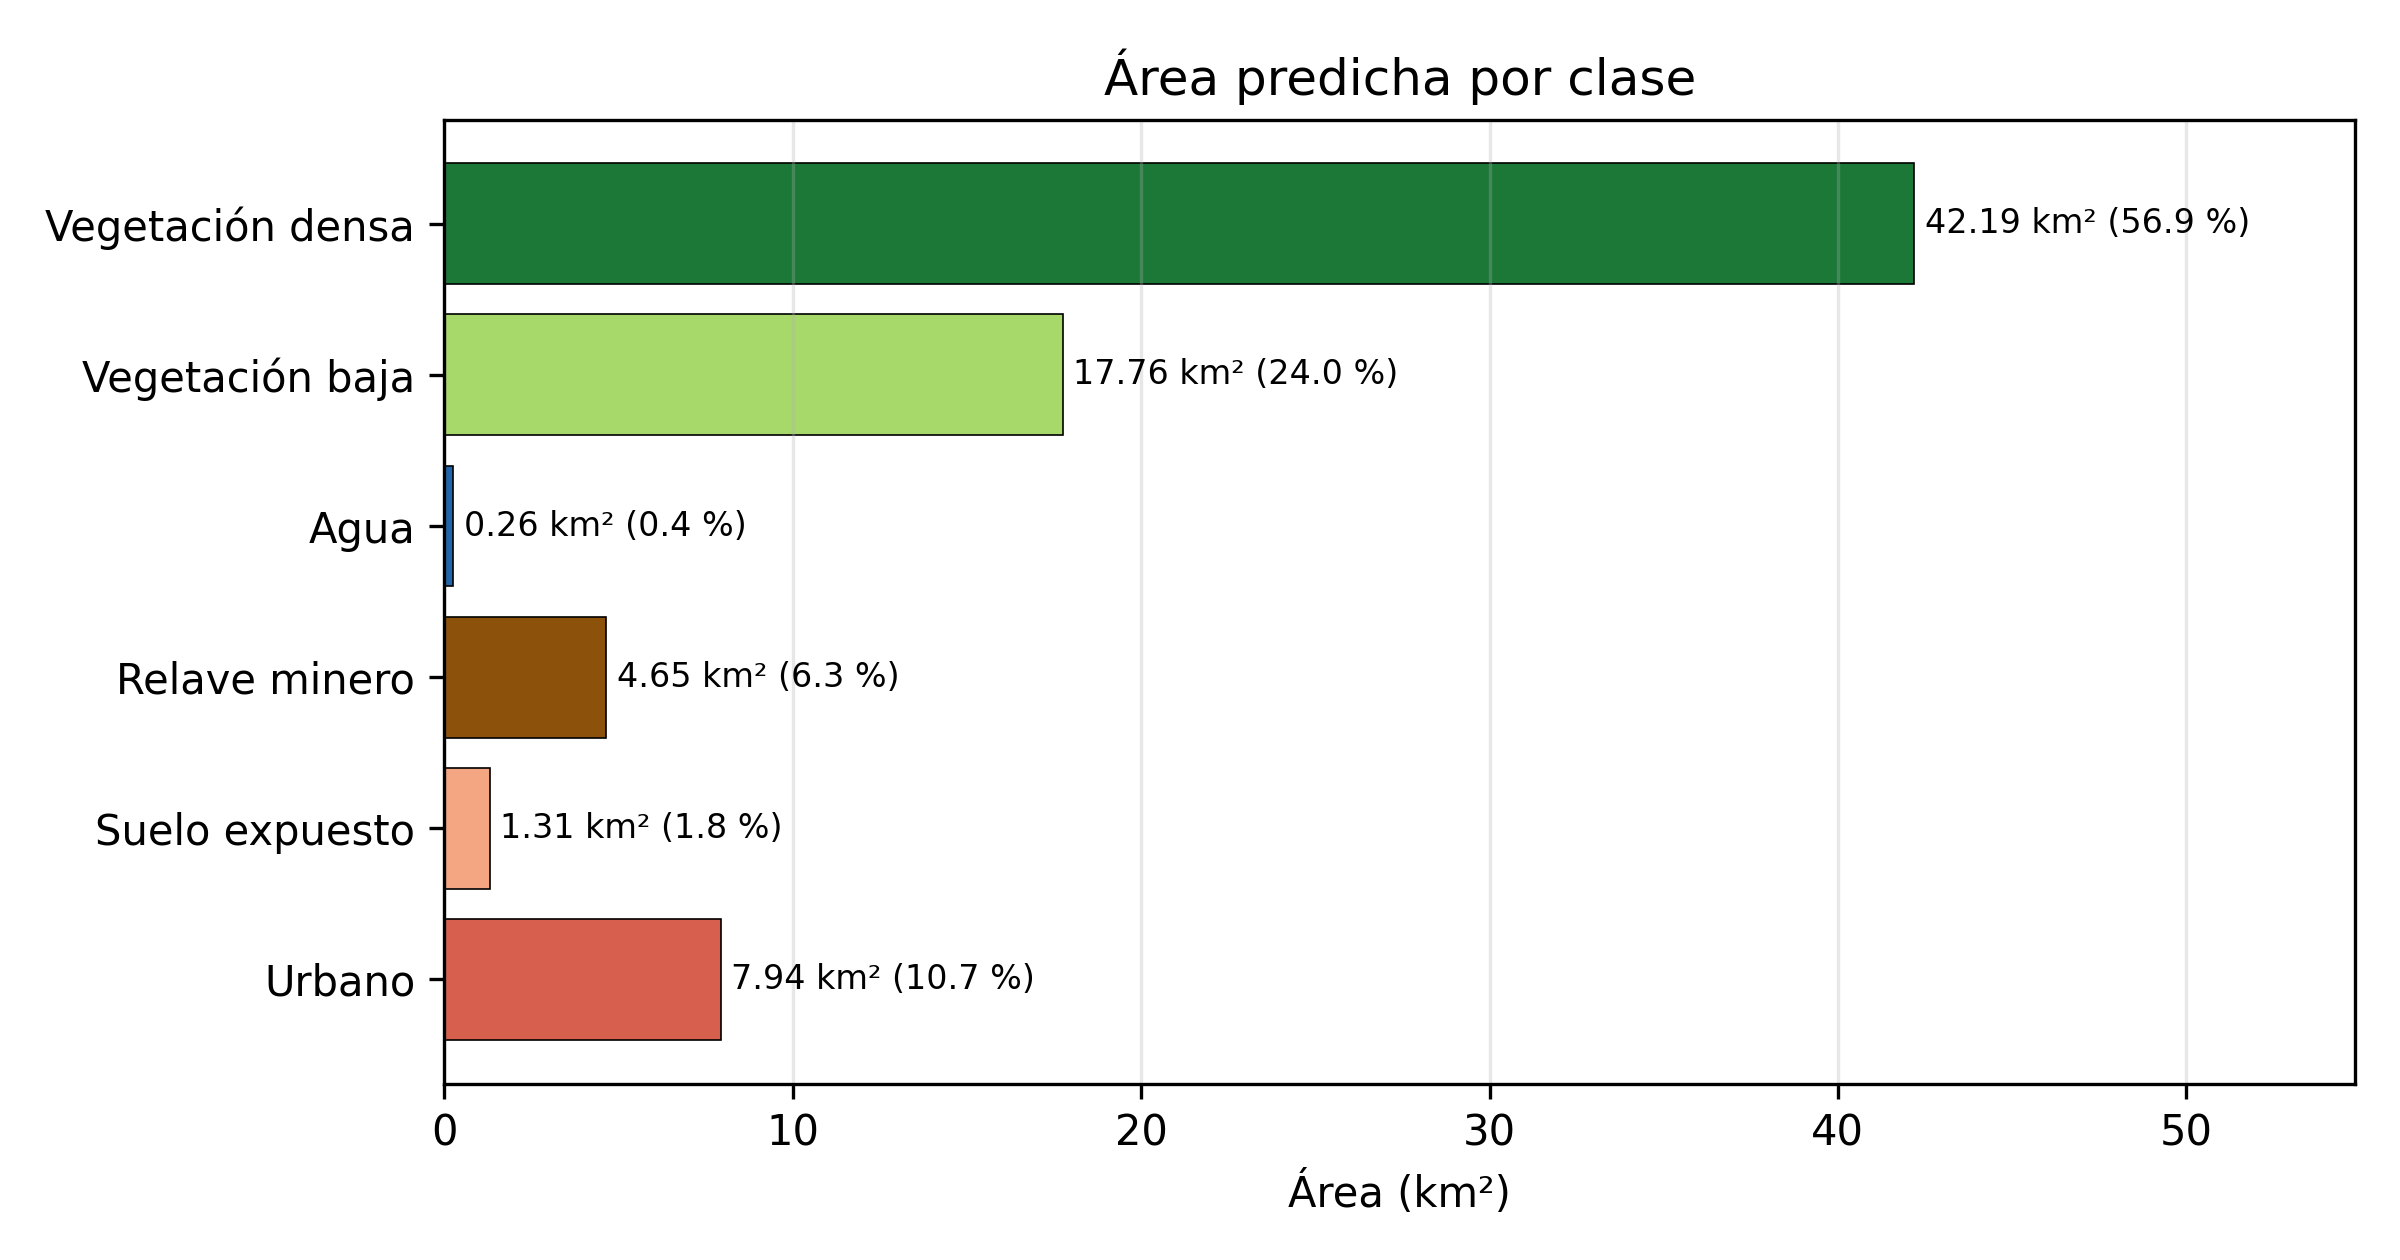
\includegraphics[width=0.85\textwidth]{figures/area_clases.png}
 \caption{Área predicha por clase sobre el área válida.}
 \label{fig:area}
\end{figure}

\begin{sloppypar}
La vegetación densa ocupa 42{,}19\,km$^2$ (56{,}9\,\% del área válida), la vegetación baja 17{,}76\,km$^2$ (24{,}0\,\%), el urbano 7{,}94\,km$^2$ (10{,}7\,\%), el relave 4{,}65\,km$^2$ (6{,}3\,\%), el suelo expuesto 1{,}31\,km$^2$ (1{,}8\,\%) y el agua 0{,}26\,km$^2$ (0{,}4\,\%).
\end{sloppypar}

La clase relave requiere una lectura cuidadosa. El corredor del relave tiene 5{,}38\,km$^2$; el modelo predice 2{,}85\,km$^2$ de relave dentro del corredor y 1{,}80\,km$^2$ fuera. El área total de 4{,}65\,km$^2$ no debe interpretarse como el volumen o la extensión oficial del lodo: el modelo confunde parte de las superficies mineras desnudas con relave. La Tabla~\ref{tab:area_corredor} separa la predicción dentro del corredor.

\begin{table}[htbp]
 \centering
 \small
 \setlength{\tabcolsep}{4pt}
 \caption{Área predicha dentro del corredor del relave. El corredor tiene 5{,}38\,km$^2$; el resto de la clase relave queda fuera de sus límites.}
 \label{tab:area_corredor}
 \begin{tabular}{lcc}
  \toprule
  Clase & Píxeles & km² \\
  \midrule
  Vegetación densa & 19.516 & 1{,}952 \\
  Vegetación baja & 2.277 & 0{,}228 \\
  Agua & 828 & 0{,}083 \\
  Relave minero & 28.537 & 2{,}854 \\
  Suelo expuesto & 885 & 0{,}088 \\
  Urbano & 1.675 & 0{,}168 \\
  \bottomrule
 \end{tabular}
\end{table}


\section{Discusión}

El mapa es coherente con la escena: la vegetación domina el área, el urbano se concentra en el casco de Brumadinho, el agua aparece en lagunas y cauces, y el relave sigue el valle del Ribeirão Ferro-Carvão. La separación de vegetación, agua y relave es alta en el test. La dificultad está en suelo expuesto y urbano: sus firmas son parecidas y, a 10\,m, un polígono de suelo puede contener lotes, vías o materiales de construcción. El error de \texttt{5\_06} es consistente con esa ambigüedad: no es un píxel aislado, es un polígono completo.

La ampliación del dataset no mejora de forma demostrable el desempeño. El mejor resultado de la Fase~3 sigue siendo 94{,}7\,\% de exactitud y 0{,}935 de Kappa, igual que la línea base de la Fase~2. La búsqueda de hiperparámetros encontró configuraciones con Kappa de validación más alto, pero no generalizaron mejor al test. En un conjunto de 24 polígonos, una diferencia de uno o dos polígonos cambia varios puntos porcentuales.

Quedan limitaciones importantes:

\begin{itemize}
 \item las etiquetas son pseudo-etiquetas construidas con reglas espectrales y revisión visual, no verdad de campo;
 \item los 72 polígonos originales y los candidatos de suelo no tuvieron revisión individual;
 \item el test tiene solo 24 polígonos y los intervalos bootstrap son amplios;
 \item cinco polígonos añadidos quedaron a 10--60\,m de polígonos de prueba, por debajo de la separación mínima de la Fase~1;
 \item el mapa usa una sola fecha y una sola escena; no captura cambios temporales ni valida la persistencia de las clases;
 \item la clase relave se confunde con superficies mineras desnudas fuera del corredor.
\end{itemize}

\section{Conclusiones}

\begin{enumerate}
 \item La regresión logística regularizada con pesos balanceados fue el modelo más estable; su test es 0{,}947 de exactitud y 0{,}935 de Kappa.
 \item El HPO no produjo una mejora demostrable frente a la Fase~2; el valor de la fase está en el protocolo de selección y en la inferencia completa, no en un aumento artificial de las métricas.
 \item El GeoTIFF temático conserva la grilla, el CRS y el \emph{transform} de la imagen, y puede abrirse y simbolizarse en QGIS.
 \item El área válida es 74{,}10\,km$^2$; la vegetación densa y baja dominan, y el relave predicho es 4{,}65\,km$^2$, de los cuales 2{,}85\,km$^2$ están dentro del corredor.
 \item La estimación de relave y suelo es la parte más débil del mapa; antes de usarla como inventario se necesita verdad de campo y una revisión de las etiquetas.
\end{enumerate}

\section{Reproducibilidad}

El flujo completo se ejecuta con el entorno de \texttt{requirements.txt}. Los scripts de la Fase~3 son:

\begin{table}[htbp]
 \centering
 \small
 \begin{tabularx}{\textwidth}{lX}
  \toprule
  Script & Función \\
  \midrule
  \texttt{05\_tune\_models.py} & HPO agrupado, selección, test, bootstrap y modelo final. \\
  \texttt{06\_predict\_raster.py} & Inferencia por bloques, GeoTIFF, estilo QML y áreas. \\
  \texttt{07\_phase3\_figures.py} & Figuras y tablas de la fase. \\
  \texttt{07b\_qgis\_map.py} & Proyecto QGIS y exportación del mapa. \\
  \texttt{08\_validate\_phase3.py} & Validación del split, el modelo, el ráster y las áreas. \\
  \bottomrule
 \end{tabularx}
\end{table}

Los comandos son:

\begin{verbatim}
run.bat src\05_tune_models.py
run.bat src\06_predict_raster.py
run.bat src\07_phase3_figures.py
run_qgis.bat src\07b_qgis_map.py
run.bat src\08_validate_phase3.py
latexmk -pdf -interaction=nonstopmode -halt-on-error main.tex
\end{verbatim}

Los artefactos principales son:
\begin{itemize}
 \item \texttt{models/final\_model.joblib} y \texttt{models/model\_card.json};
 \item \texttt{data/prediction/landcover\_lr.tif};
 \item \texttt{data/prediction/landcover\_lr.qml};
 \item \texttt{results/phase3\_*.csv}.
\end{itemize}
La imagen original, la SCL y los polígonos se conservan en \texttt{data/}.

\printbibliography

\end{document}
